% arara: pdflatex
%        File: LinearAlgebra.tex
%     Created: Fri Jun 09 06:00 PM 2023 B
% Last Change: Fri Jun 09 06:00 PM 2023 B
%
\documentclass[12pt, a4paper]{article}

\usepackage[]{amsmath}
\usepackage{amssymb}
\usepackage{amsthm}
\usepackage{mathtools}
\usepackage[]{hyperref}
\usepackage{caption}
\usepackage{subcaption}
\usepackage[]{graphicx}
\graphicspath{ {./imgs/} }

% Augmented Matrix (Argument is one less than the number of columns)
\newenvironment{amatrix}[1]{%
  \left(\begin{array}{@{}*{#1}{c}|c@{}}
}{%
  \end{array}\right)
}

\newcommand{\R}{\mathbb{R}}
\newcommand{\spantext}{\text{span}}
\newcommand{\inner}[1]{\langle #1 \rangle}
\newcommand{\norm}[1]{\lvert \lvert #1 \rvert \rvert}
\newcommand{\intd}{\,\text{d}}

\renewcommand{\labelitemii}{$\circ$}

\DeclareMathOperator{\im}{Im}
\DeclareMathOperator{\Null}{null}
\DeclareMathOperator{\Rank}{rank}
\DeclareMathOperator{\sgn}{sgn}
\DeclareMathOperator{\tr}{tr}
\DeclareMathOperator{\diag}{diag}

\theoremstyle{remark}
\newtheorem{remark}{Remark}
\theoremstyle{definition}
\newtheorem{definition}{Definition}
\newtheorem{example}{Example}
\newtheorem{exercise}{Exercise}

\numberwithin{equation}{section}
\numberwithin{definition}{section}
\numberwithin{example}{section}
\numberwithin{exercise}{section}
\numberwithin{remark}{section}
\numberwithin{figure}{section}
\title{Linear Algebra I \& II Summary}
\author{Paul Kim}
\begin{document}
\maketitle

\section*{Preface}
Note that this is not your actual lecture note,
and I do not condone only sticking to this as your resource.
On the other hand, if you are reading this for your intuition,
you are at the right place.

This document is based on 2019 linear algebra I and 2018 linear algebra II lecture notes by Vicky Neale and Ulrike Tillmann.
You can check them out at \url{https://courses.maths.ox.ac.uk/} in the Archive tab.

Most examples here will include the ones from these lecture notes.

Note that this summary note will gloss over quite many of the proofs, but will try to give general intuition behind them.

\newpage
\part{Linear Algebra I}
\newpage

\section{Linear Equations and Matrices}
You've probably already seen linear system of equations like the following:
\begin{align}
    &
    \begin{cases}
        3x + 5y = -1 \\
        4x - y = 10
    \end{cases}
    \label{equ: Linear Equation 1}
    \\
    &
    \begin{cases}
        2x + y = 0 \\
        4x + 2y = 1
    \end{cases}
    \label{equ: Linear Equation 2}
    \\
    &
    \begin{cases}
        8x - 7y + 6z = 59 \\
        x + 2z = 9 \\
        3x + 2y - z = 11
    \end{cases}
    \label{equ: Linear Equation 3}
\end{align}
Note that (\ref{equ: Linear Equation 1}) and (\ref{equ: Linear Equation 3}) are uniquely solvable, but (\ref{equ: Linear Equation 2}) does not have solution.

You've probably also seen examples of ones with infinite solutions (because for example, you have more variables than ``effective'' equations).

You can analyze them by hand, but is there a systematic approach to analyzing them?
Say, you are telling a computer to solve these. What are your options?

\begin{definition}[Matrix]
    For $m,n \geq 1$, an \underline{$m \times n$ matrix} is a rectangular array with $m$ rows and $n$ columns with entries from $\R$ (or $\mathbb{C}$ or other fields).
\end{definition}
\begin{remark}
    \textbf{Always count the number of rows, then number of columns}.
\end{remark}
\begin{remark}
    Notation: For matrix $A \in \R^{m \times n}$, $A_{i,j}$ represents the entry at row $i$ and column $j$.
\end{remark}
\begin{example}[Matrices]
    Here are examples of $3 \times 2$ matrices:
    \begin{align*}
        &
        \begin{pmatrix}
            3 & 2 & 1 \\
            1 & -2/3 & 0
        \end{pmatrix} \\
        &
        \begin{pmatrix}
            0 & 0 & 0 \\
            i & 0 & 0
        \end{pmatrix}
    \end{align*}
\end{example}
\begin{definition}[Vector]
    An $n \times 1$ matrix is called a \textbf{column vector}.
    A $1 \times n$ matrix is called a \textbf{row vector}.
\end{definition}
\begin{example}[Vector]
    Here are examples of a column vector and a row vector respectively:
    \begin{align*}
        &
    \begin{pmatrix}
        1 \\
        0 \\
        -1
    \end{pmatrix}
    \\
    &
    \begin{pmatrix}
        1 & 3 & 2 & 5
    \end{pmatrix}
    \end{align*}
\end{example}
\begin{remark}
    \label{rmk: Column Vector}
    \textbf{I highly recommend using variables for denoting column vectors by default}.
    For example $v = 
    \begin{pmatrix}
        1 \\ 2
    \end{pmatrix}
    $
    If you get a row vector, always denote it with a transpose: $ v^T =
    \begin{pmatrix}
        1 & 2
    \end{pmatrix}
    $
    This is because by convention, we will use left multiplication by a matrix far more often then right multiplication.
\end{remark}
\begin{definition}[Square Matrices]
    A matrix with the same number of rows and columns is called a \textbf{square matrix}.
\end{definition}

\subsection{Matrix Multiplication and Transpose}
Addition and subtractions: $A + B$ are defined naturally by their entry-wise operation. (Note that $A$ and $B$ have to have the same dimensions!)
Multiplication of matrices $A$ and $B$ are defined for $A \in \R^{m \times n}$, $B \in \R^{n \times \ell}$ as the following
\begin{definition}[Matrix Multiplication]
    \begin{equation*}
        \left( A B \right)_{i, j} = \sum_{k = 1}^{n} \left( A_{i,k} \right) \left( B_{k,j} \right)
    \end{equation*}
    Note that the resulting $AB$ has dimension $m \times \ell$.
\end{definition}
\begin{example}[Matrix Multiplication]
    Consider the following two matrices:
    \begin{align*}
        A &=
        \underbrace{
        \begin{pmatrix}
            3 & 1 & 2 \\
            4 & 5 & -1
    \end{pmatrix}}_{2 \times 3} \\
        B &=
        \underbrace{
        \begin{pmatrix}
            10 \\
            15 \\
            -5
        \end{pmatrix}
    }_{3 \times 1}
    \end{align*}
    Then:
    \begin{equation*}
        AB = 
        \underbrace{
        \begin{pmatrix}
            3 & 1 & 2 \\
            4 & 5 & -1
    \end{pmatrix}}_{2 \times 3}
        \underbrace{
        \begin{pmatrix}
            10 \\
            15 \\
            -5
        \end{pmatrix}
    }_{3 \times 1}
    =
    \underbrace{
    \begin{pmatrix}
        3 \times 10 + 1 \times 15 + 2 \times (-5) \\
        4 \times 10 + 5 \times 15 + (-1) \times (-5)
    \end{pmatrix}
}_{2 \times 1}
    \end{equation*}
\end{example}
\begin{remark}
    One way to remember if matrix multiplication is well-defined is to note that:
    $m \times$ \underline{$n$} and \underline{$n$} $\times \ell$ results in $m \times \ell$.
\end{remark}
\begin{remark}
    The way matrix multiplication is defined may not be intuitive.
    However, it is a natural way to capture \textit{linear transforms}.
\end{remark}
\begin{exercise}[Associativity of Matrix Multiplication]
    Show that for $A \in \R^{m \times n}$, $B \in \R^{n \times \ell}$, and $C \in \R^{\ell \times p}$, then $(AB)C = A(BC)$. Is it true that $AB=BA$ in general?
\end{exercise}
\begin{remark}[Submatrix Multiplication]
    \textbf{Pro tip!}
    If you can identify two matrices in the form of:
    \begin{align*}
        A &= 
        \begin{pmatrix}
            A_{11} & A_{12} \\ A_{21} & A_{22}
        \end{pmatrix} \\
        B &= 
        \begin{pmatrix}
            B_{11} & B_{12} \\ B_{21} & B_{22}
        \end{pmatrix}
    \end{align*}
    or otherwise, then you can compute multiplication by performing ``submatrix multiplication'':
    \begin{equation*}
        AB = 
        \begin{pmatrix}
            A_{11} & A_{12} \\ A_{21} & A_{22}
        \end{pmatrix} 
        \begin{pmatrix}
            B_{11} & B_{12} \\ B_{21} & B_{22}
        \end{pmatrix}
        =
        \begin{pmatrix}
            A_{11}B_{11} + A_{12}B_{21} & A_{11} B_{12} + A_{12} B_{22} \\
            A_{21}B_{11} + A_{22}B_{21} & A_{21} B_{12} + A_{22} B_{22}
        \end{pmatrix}
    \end{equation*}
    \underline{so long as the matrix multiplications are defined}.

    This is useful in situations such as:
    \begin{equation*}
        A
        \underbrace{
        \begin{pmatrix}
            b_1 & b_2 & \cdots & b_n
    \end{pmatrix}}
    _{B}
    =
    \begin{pmatrix}
        Ab_1 & Ab_2 & \cdots Ab_n
    \end{pmatrix}
    \end{equation*}
    where $b_i$ are the columns of $B$.
\end{remark}
\begin{exercise}[Diagonal matrices form a ring]
    Show that for \textbf{diagonal matrices} $A \in \R^{n \times n}$ and $B \in \R^{n \times n}$ such that $A_{i,j} = B_{i,j} = 0$ for $i \neq j$, $AB$ should also be a diagonal matrix.
\end{exercise}
\begin{exercise}[Triangular matrices form a ring]
    Show that for \textbf{upper triangular} $A \in \R^{n \times n}$ and $B \in \R^{n \times n}$ such that $A_{i,j} = B_{i,j} = 0$ for $i > j$, $AB$ should also be an upper triangular matrix.
\end{exercise}
\begin{exercise}
    How many diagonal $A \in \R^{n \times n}$ are there such that
    \begin{equation*}
        A^2 = I
    \end{equation*}
    where $I$ is the \textbf{identity matrix}, a diagonal matrix with only 1s in the diagonal entry.
\end{exercise}
\begin{definition}[Transpose]
    For $A \in \R^{m \times n}$, \textbf{transpose} $A^T \in \R^{n \times m}$ is defined as
    \begin{equation*}
        \left( A^T \right)_{i,j} = A_{j,i}
    \end{equation*}
\end{definition}
\begin{example}[Transpose]
    \begin{equation*}
        \begin{pmatrix}
            3 & 0 & 1 \\
            4 & 2 & 5
        \end{pmatrix}^T
        =
        \begin{pmatrix}
            3 & 4 \\
            0 & 2 \\
            1 & 5
        \end{pmatrix}
    \end{equation*}
\end{example}
\begin{remark}
    \begin{itemize}
            \item Taking transpose of a row vector turns it into a column vector.
            \item Taking a transpose of a column vector turns it into a row vector.
            \item For any $A \in \R^{m \times n}$, $\left( A^T \right)^T = A$
    \end{itemize}
\end{remark}
\begin{exercise}[Symmetric Triangular Matrix is Diagonal]
    Show that if an upper triangular matrix $A \in \R^{n \times n}$ satisfies $A^T = A$, then it must be a diagonal matrix.
\end{exercise}
\begin{exercise}[Antisymmetric Matrix Does Not Have Diagonal Entries]
    Show that if $A \in \R^{n \times n}$ satisfies $A^T = -A$, then $A_{i,i} = 0$ for all $i = 1, \cdots n$.
\end{exercise}
\begin{exercise}[Transpose of Product of Matrix]
    Show that for any $A \in \R^{m \times n}$ and $B \in \R^{n \times \ell}$,
    \begin{equation*}
        \left( AB \right)^T = B^T A^T
    \end{equation*}
    Using this result, show that product of two symmetric matrices ($A^T = A$) is also a symmetric matrix.
\end{exercise}
\begin{remark}
    For two column vectors $v_1$ and $v_2$, the dot product can be written as $v_1^T v_2$.
    This becomes a useful notation for dot product, in factf
    \footnote{
    Technically $1 \times 1$ matrix, but there is no problem in taking that as just a scalar.}
\end{remark}

\section{System of Simultaneous Linear Equations to Matrix Equations}
We've seen a system like (\ref{equ: Linear Equation 1}), (\ref{equ: Linear Equation 2}), and (\ref{equ: Linear Equation 3}).

We can turn the three examples of linear system of equations to the following \textbf{matrix equations} of the form $\underbrace{A}_{\text{Matrix}}\underbrace{x}_{\text{Column Vector}} = \underbrace{b}_{\text{Column Vector}}$:
\begin{align}
    &
    \begin{pmatrix}
        3 & 5 \\
        4 & -1
    \end{pmatrix}
    \begin{pmatrix}
        x \\ y
    \end{pmatrix}
    &=
    \begin{pmatrix}
        -1 \\ 10
    \end{pmatrix}
    \\
    &
    \begin{pmatrix}
        2 & 1 \\
        4 & 2
    \end{pmatrix}
    \begin{pmatrix}
        x \\ y
    \end{pmatrix}
    &= 
    \begin{pmatrix}
        0 \\ 1
    \end{pmatrix}
    \\
    &
    \begin{pmatrix}
        8 & -7 & 6 \\
        1 & 0 & 2 \\
        3 & 2 & -1
    \end{pmatrix}
    \begin{pmatrix}
        x \\ y \\ z
    \end{pmatrix}
    &=
    \begin{pmatrix}
        59 \\ 9 \\ 11
    \end{pmatrix}
\end{align}

One could do even better and skip writing the name of the variables:
\begin{align}
    &
    \begin{amatrix}{2}
        3 & 5 & -1 \\
        4 & -1 & 10
    \end{amatrix}
    \\
    &
    \begin{amatrix}{2}
        2 & 1 & 0 \\
        4 & 2 & 1
    \end{amatrix}
    \\
    &
    \begin{amatrix}{3}
        8 & -7 & 6 & 59 \\
        1 & 0 & 2 & 9 \\
        3 & 2 & -1 & 11
    \end{amatrix}
\end{align}
(the bar is decorative to show that the system is augmented.)

Our task is to solve it, that is, we wish to put $\left( A \middle| b \right)$ into the form $\left( I \middle| \tilde b \right)$.
This is unfortunately not possible to do\footnote{
A colloquial saying is that with $n$ variables to solve, you need $n$ independent equations.}.

For example, the following system is over-determined (more equations\footnote{Conditions} than variables):
\begin{equation*}
    \begin{cases}
    3x + y = -4 \\
    2x - 5y = 3 \\
    x + 2y = 8
    \end{cases}
\end{equation*}
and the following is under-determined (less equations than variables):
\begin{equation*}
    \begin{cases}
        x + 2y = 5
    \end{cases}
\end{equation*}
Also (\ref{equ: Linear Equation 2}) is an inconsistent system, as the two equations violate each other.
As you could see, \underline{there are many ways things can go wrong}.

A systematic approach to make analysis easier by performing ``row operations'' is the \textbf{Gaussian elimination}.

\section{EROs and Gaussian Elimination}
\begin{definition}[Elementary Row Operations (ERO)]
    For a matrix $A \in \R^{m \times n}$, following are the three elementary row operations.
    \begin{itemize}
        \item For $1 \leq r < s \leq m$, $R_s \leftrightarrow R_r$ (Exchange row $r$ and row $s$)
        \item For $1 \leq r \leq m$ and $\lambda \neq 0$, $R_r \rightarrow \lambda R_r$ (Multiply row $r$ by $\lambda$)
        \item For $1 \leq r, s \leq m$ where $r \neq s$ and $\lambda \in \mathbb{F}$, $R_s \rightarrow R_s + \lambda R_r$ (Add to row $s$ the row $r$ multiplied by $\lambda$)
    \end{itemize}
\end{definition}
\begin{remark}
    It is \textbf{paramount} that each operation is reversible.
\end{remark}
\begin{remark}
    It is \textbf{recommended} that you do not compose bunch of EROs as one ERO, as tempting as it is.
    Using pure EROs is useful for determinant analysis later.
\end{remark}
Now we need the notion of ``simplified'' matrix under these operations.
\begin{definition}[Echelon Form]
    $M \in \R^{m \times n}$ is in \textbf{echelon form} if
    \begin{itemize}
        \item If row $r$ of $M$ has any nonzero entries, the first of these is 1.
        \item If $1 \leq r < s \leq m$, and row $r$ and row $s$ contain nonzero entries ($M_{r,j}$ and $M_{s, k}$ respectively), then $j < k$.
            \begin{itemize}
                \item ``Leading entry of lower rows should come to the right of the ones on the higher rows.''
            \end{itemize}
        \item If row $r$ of $M$ contains nonzero entries and row $s$ does not, then $r < s$
            \begin{itemize}
                \item ``Zero rows are below all nonzero rows.''
            \end{itemize}
    \end{itemize}
\end{definition}
\begin{example}[Echelon Form]
    The following matrix in echelon form:
    \begin{equation*}
        \begin{pmatrix}
            1 & 2 & 3 & 4 & 2 \\
            0 & 1 & 2 & 3 & 0 \\
            0 & 0 & 0 & 0 & 1
        \end{pmatrix}
    \end{equation*}
\end{example}
\subsection{Gaussian Elimination}
Now we need an algorithm to perform Gaussian elimination to reduce matrix.
The idea is to take a matrix $A$, and eliminate the leading order entries one by one to echelon form.
\begin{example}[Gaussian Elimination]
    \begin{align*}
        \begin{amatrix}{2}
            3 & 5 & -1 \\
            4 & -1 & 10
        \end{amatrix}
        & \xrightarrow{\substack{R_1 \rightarrow \frac{1}{3} R_1 \\ R_2 \rightarrow \frac{1}{4} R_2}}
        \begin{amatrix}{2}
            1 & \frac{5}{3} & -\frac{1}{3} \\
            1 & -\frac{1}{4} & \frac{5}{2}
        \end{amatrix}
        \\
        & \xrightarrow{R_2 \rightarrow R_2 - R1}
        \begin{amatrix}{2}
            1 & \frac{5}{3} & -\frac{1}{3} \\
            0 & -\frac{23}{12} & \frac{17}{6}
        \end{amatrix} \\
        & \xrightarrow{R_2 \rightarrow -\frac{12}{23}R_2}
        \underbrace{
        \begin{amatrix}{2}
            1 & \frac{5}{3} & -\frac{1}{3} \\
            0 & 1 & -\frac{34}{23}
    \end{amatrix}}_{\text{echelon}}
    \end{align*}
\end{example}
\begin{remark}
    If there was a zero in the leading entry of the first column, one could swap the rows.
\end{remark}
\begin{example}[Gaussian Elimination (Cont'd)]
    We could take it even further and get \textbf{reduced row echelon (RRE) form}.
    \begin{align*}
        \begin{amatrix}{2}
            1 & \frac{5}{3} & -\frac{1}{3} \\
            0 & 1 & -\frac{34}{23}
        \end{amatrix}
        & \xrightarrow{R_1 \rightarrow R_1 - \frac{5}{3}R_2}
        \underbrace{
        \begin{amatrix}{2}
            1 & 0 & -\frac{49}{23} \\
            0 & 1 & \frac{34}{23}
    \end{amatrix}}_{\text{RRE}}
    \end{align*}
    So $x = -\frac{49}{23}$ and $y = \frac{34}{23}$ for (\ref{equ: Linear Equation 1}).
\end{example}
\begin{exercise}
    Given $A \in \R^{n \times n}$, show that it can be reduced to RRE within $n^2$ EROs.
\end{exercise}
\subsection{Inverse Matrix}
\begin{definition}[Inverse Matrix]
    Note that if it is possible to identify $B \in \R^{n \times n}$ such that $AB = BA = I$, then we call this $B$ the \textbf{inverse matrix} of $A$, and write $A^{-1} \coloneqq B$.
    We also say that $A$ is invertible in this case.
\end{definition}
\begin{remark}
    For a well-posed matrix equation $Ax = b$ where $A \in \R^{n \times n}$ being an invertible matrix,
    one could write the solution as $x = A^{-1} b$.
\end{remark}
\begin{exercise}[Inverse is Unique]
    If $A \in \R^{n \times n}$ is invertible, show that the inverse $A^{-1}$ is well-defined.
\end{exercise}
\begin{exercise}[Inverse of Product]
    If $A,B \in \R^{n \times n}$ are both invertible matrices, then show that
    \begin{equation*}
        \left( AB \right)^{-1} = B^{-1}A^{-1}
    \end{equation*}
\end{exercise}
\begin{exercise}[Inverse Transpose]
    If $A \in \R^{n \times n}$ is invertible, then show that $A^{T}$ is also invertible,
    and that:
    \begin{equation*}
        \left( A^T \right)^{-1} = \left( A^{-1} \right)^T
    \end{equation*}
\end{exercise}
\begin{remark}
    The above exercise shows that one could write $A^{-T}$ as a shorthand for inverse transpose of $A$.
\end{remark}
It is possible to compute the inverse matrix (should it exist) via Gaussian elimination.
Consider $A \in \R^{n \times n}$, an invertible matrix.
Perform Gaussian elimination on $\left( A \middle| I \right) \in \R^{n \times 2n}$, then we should end up with:
$\left( I \middle| A^{-1} \right)$.
\begin{remark}
    For the proof, refer to the actual lecture note. Try showing that if $A \in \R^{n \times n}$ is invertible, then RRE is the identity matrix.
\end{remark}
\begin{remark}
    In practice, computing the inverse matrix is in fact not a feasible thing to do (considering data sets are enormous, and we are often only interested in solution to one single solution to a matrix equation).
\end{remark}
\subsection{Special Square Matrices}
Here is a list of some notable matrices, some of which are already mentioned:
\begin{itemize}
    \item $I \in \R^{n \times n}$ such that $I_{ij} = \delta_{i,j}$ is an identity matrix.
    \item $T \in \R^{n \times n}$ such that $T_{i,j} = 0$ for $i > j$ is an upper triangular matrix.
    \item $T \in \R^{n \times n}$ such that $T_{i,j} = 0$ for $i < j$ is a lower triangular matrix.
    \item $Q \in \R^{n \times n}$ such that $Q^T Q = I = Q Q^T$ is an orthogonal matrix.
    \item $A \in \R^{n \times n}$ such that $A^T = A$ is a symmetric matrix.
    \item $B \in \R^{n \times n}$ such that $B^T = -B$ is an antisymmetric matrix.
    \item $U \in \mathbb{C}^{n \times n}$ such that $U^* U = I = U U^*$ is a unitary matrix\footnote{The star denotes conjugate transpose}.
\end{itemize}
\section{Vector Spaces}
\begin{definition}[Vector Space]
    Let $\mathbb{F}$ be a field. A \textbf{vector space} over $\mathbb{F}$ is a non-empty set $V$ with
    addition and scalar multiplication operation defined, satisfying the vector space axioms:
    \begin{itemize}
        \item Addition is commutative.
            \begin{itemize}
                \item $u + v = v + u$.
            \end{itemize}
        \item Addition is associative.
            \begin{itemize}
                \item $\left( u + v \right) + w = u + \left( v + w \right)$
            \end{itemize}
        \item There exists an additive identity.
            \begin{itemize}
                \item $0 \in V$
            \end{itemize}
        \item There exists additive inverse for every element.
            \begin{itemize}
                \item $\forall v \in V: \exists (-v) \in V$
            \end{itemize}
        \item Scalar multiplication is distributive over vector addition.
            \begin{itemize}
                \item $\lambda \left( u + v \right) = \lambda u + \lambda v$
            \end{itemize}
        \item Scalar multiplication is distributive over scalar multiplication.
            \begin{itemize}
                \item $\left( \lambda + \mu \right) v = \lambda v + \mu v$
            \end{itemize}
        \item Scalar multiplication interacts well with field multiplication.
            \begin{itemize}
                \item $\left( \lambda \mu \right) v = \lambda \left( \mu v \right)$
            \end{itemize}
        \item Identity for scalar multiplication.
            \begin{itemize}
                \item $1v = v$
            \end{itemize}
    \end{itemize}
\end{definition}
\begin{example}[Vector Space: $\R^n$]
    $\R^n$ is a vector space.
    Honestly, this is the most important vector space, so I suggest you get used to working in here.
    Note that often you can restrict your attention to $\R^3$, and most of your intuition also applies in higher dimensions.
\end{example}
\begin{example}[Other Vector Spaces]
    Other vector spaces include:
    \begin{itemize}
        \item $\mathbb{C}$ is a vector space over field $\R$ (essentially $\mathbb{C}$ is the same thing as $\R^2$).
        \item $\mathcal{P}_n$, the space of polynomials of degree $n$ or less is a vector space over $\R$.
    \end{itemize}
\end{example}
\begin{exercise}[Uniqueness of Additive Identity and Inverse]
    For vector space $V$, 
    \begin{itemize}
            \item show that the additive identity element is unique.
            \item show that for any $v \in V$, the additive inverse $(-v)$ is well-defined.
    \end{itemize}
\end{exercise}
\begin{definition}[Subspaces]
    Let $V$ be a vector space over $\mathbb{F}$. $U \subset V$ is a \textbf{subspace} of $V$ if it is nonempty, closed under addition and scalar multiplication.
\end{definition}
\begin{exercise}[Subspace Test]
    Let $V$ be a vector space over $\mathbb{F}$.
    Let $U$ be a subset of $V$.
    Show that $U$ is a subspace of $V$ if and only if $0 \in U$ and $\lambda u_1 + u_2 \in U$ for all $u_1, u_2 \in U$ and $\lambda \in \mathbb{F}$.
\end{exercise}
\begin{remark}
    If you think about subspace test for a long time, it kinda becomes obvious; the fact that $\lambda u_1 + u_2 \in U$ captures the idea of closure under both addition and scalar multiplication.
\end{remark}
\begin{exercise}[Subspace is also a Vector Space]
    If $V$ is a vector space and $U$ is a subspace of $V$,
    show that
    \begin{itemize}
        \item $U$ is a vector space.
        \item If $W$ is a subspace of $U$, then $W$ is a subspace of $V$.
    \end{itemize}
\end{exercise}
\begin{example}[Hyperplane is a Subspace of $\R^n$]
    $U \coloneqq \left\{ \left( x,y,z \right) \in \R^3 \middle| x + 2y + z = 0\right\} \leq \R^3$.
    \begin{figure}[h]
        \centering
        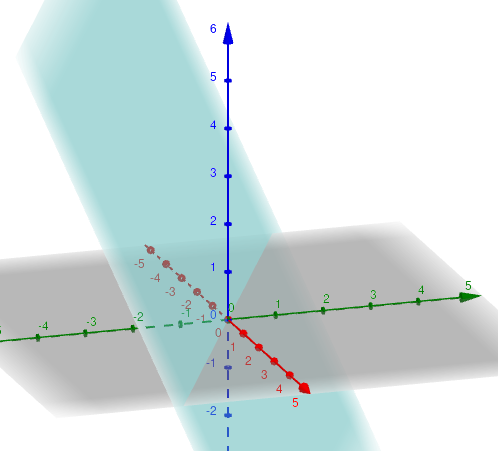
\includegraphics[scale=0.2]{hyperplane121}
        \caption{$x + 2y + z = 0$}
    \end{figure}
\end{example}
\begin{definition}[Sum Space]
    For $A,B \subset V$ where $V$ is a vector space, define $A + B \coloneqq \left\{ a + b \middle| a\in A, b \in B \right\}$
\end{definition}
\begin{exercise}[Sum Space and Intersection are Subspaces]
    For $V$ vector space, and $U,W \leq V$, show that
    \begin{itemize}
        \item $U + W$ is a subspace of $V$.
        \item $U \cap W$ is a subspace of $V$.
    \end{itemize}
    Construct an example where $U \cup W$ is not a subspace.
\end{exercise}

\section{Bases}
\begin{definition}[Span]
    \textbf{Span} of vectors $v_1, v_2, \cdots, v_k$ is defined as $\spantext \left( \left\{ v_1, \cdots, v_k \right\} \right) \coloneqq  \left\{ \sum_{i=1}^k a_iv_i \middle| a_i \in \mathbb{F} \right\}$.
\end{definition}
\begin{example}[Span]
    Span of $\left\{ e_1, e_2 \right\}$ is $\R^2$, where $e_i$ are $i$\textsuperscript{th} canonical vector.
    Span of $\left\{ 
        \begin{pmatrix}
            1 \\ 1
        \end{pmatrix},
        \begin{pmatrix}
            1 \\ -1
        \end{pmatrix}
    \right\}$ is also $\R^2$.
\end{example}
\begin{exercise}[Span is Subspace]
    Show that span of finite number of vectors is a subspace.
\end{exercise}
\begin{definition}[Linear Combination]
    $u$ is a \textbf{linear combination} of $v_1, \cdots, v_k$ if $u \in \spantext \left( \left\{ v_1, \cdots, v_k \right\} \right)$
\end{definition}
\begin{remark}
    Note that linear combination only refers to sum of \textbf{finitely many} elements.
\end{remark}
\begin{definition}[Linear Independence]
    Let $V$ be vector space over $\mathbb{F}$.
    $v_1, \cdots, v_m \in V$ are \textbf{linearly independent} if
    $\sum_{i=1}^m \alpha_i v_i = 0$ implies $\alpha_1=\cdots=\alpha_m = 0$.
    Otherwise \textbf{linearly dependent}.
    \begin{figure}[tbp]
        \centering
        \begin{subfigure}[b]{0.45\textwidth}
            \centering
            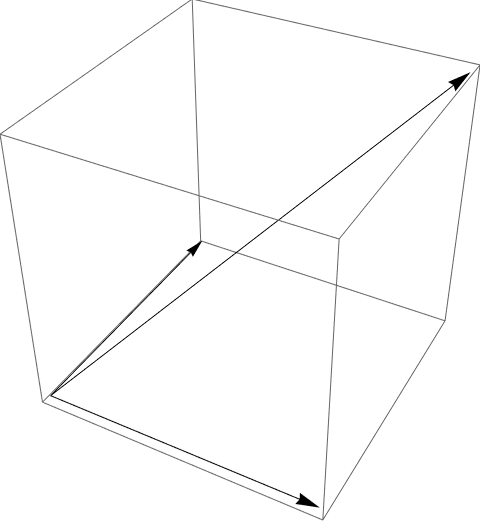
\includegraphics[width=\textwidth]{LinearIndependence}
            \caption{These three vectors are linearly independent, and they span $\R^3$.}
        \end{subfigure}
        \hfill
        \begin{subfigure}[b]{0.45\textwidth}
            \centering
            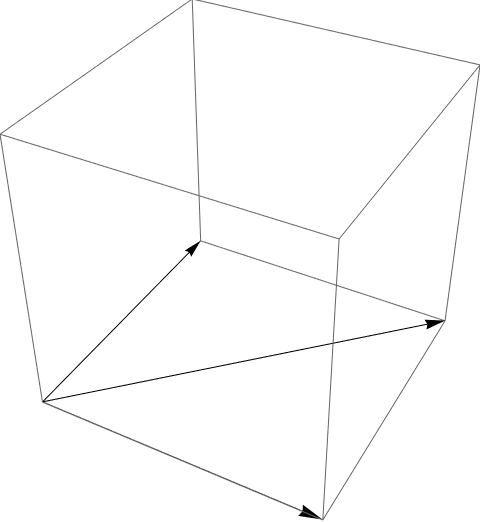
\includegraphics[width=\textwidth]{LinearDependence}
            \subcaption{Because $e_1$ and $e_2$ can be linearly combined to produce $e_1+e_2$, linearly dependent.They span $\left\{ \left( x, y, 0 \right)^T \middle| x, y \in \R \right\}$ in this case.}
        \end{subfigure}
        \caption{Linear Independence \& Linear Dependence}
        \label{fig: Linear Independence and Linear Dependence}
    \end{figure}
\end{definition}
\begin{remark}
    Might be jumping the gun a bit, but intuitionistically,
    if there are the minimal number of vectors needed to describe their span,
    they are linearly independent.
    (See Figure \ref{fig: Linear Independence and Linear Dependence})
\end{remark}
\begin{exercise}[Additional ``Nonparallel'' Vector Preserves Linear Independence]
    Suppose $v_1, \cdots, v_m$ are linearly independent in vector space $V$ over $\mathbb{F}$.
    Let $v_{m+1} \in V$ be such that $v_{m+1} \not\in \spantext \left( \left\{ v_1, \cdots, v_m \right\} \right)$.
    Show that $v_1, \cdots, v_m, v_{m+1}$ are also linearly independent.
\end{exercise}
\begin{remark}
    General strategy to showing linear independence is to assume $\sum_{i=1}^m \alpha_i v_i = 0$,
    and show that $\alpha_1 = \cdots = \alpha_{m} = 0$
\end{remark}
\begin{definition}[Bases]
    Let $V$ be a vector space. A basis of $V$ is a set of linearly independent spanning set.
\end{definition}
\begin{remark}[Basis is Nonunique]
    For $\R^3$, $\left\{ e_1, e_2, e_3 \right\}$ is a basis, but $\left\{ e_1, e_2, e_1 + e_2 + e_3 \right\}$ is also a basis.
\end{remark}
\begin{exercise}[Basis = Any Vector Has Unique Representation]
    Show that
    $\left\{ v_1, \cdots, v_n \right\} \subset V$, then
    $\left\{ v_1, \cdots, v_n \right\}$ is a basis of $V$ if and only if
    for any $v \in V$, there exists unique linear combination representation $v = \sum_{i=1}^n a_i v_i$
\end{exercise}
\begin{example}
    Suppose $v = \left( 1, 2, 3 \right)^T \in \R^3$.
    In $\left\{ e_1, e_2, e_3 \right\}$ basis, $v = 1e_1 + 2 e_2 + 3 e_3$.
    In $\left\{ \underbrace{e_1 + 2e_3}_{v_1}, \underbrace{e_2}_{v_2}, \underbrace{e_3}_{v_3} \right\}$ basis,
    $v = 1v_1 + 0v_2 + v_3$.
\end{example}
\begin{remark}[Coordinate]
    Think of the coefficients ($\alpha_i$) in the linear combination expansion $v = \sum_{i = 1}^n \alpha_i v_i$ as coordinates.
\end{remark}
\begin{exercise}[Finite Spanning Set Implies Existence of Basis]
    Show that if $V$ has finite spanning set $S$, then $S$ contains a linearly independent spanning set.
    (Hint: Let $T \subset S$ be the largest linearly independent set. Then show that $T$ spans $V$)
\end{exercise}
\begin{exercise}[Steinitz Exchange Lemma]
    Let $V$ be vector space over $\mathbb{F}$. Take $X \subset V$. Suppose $u \in \spantext \left( X \right)$,
    but $u \not\in \spantext \left( X \setminus \left\{ v \right\} \right)$ for some $V \in X$.
    Let $Y = \left( X \setminus \left\{ v \right\} \right) \cup \left\{ u \right\}$ 
    (``exchange $u$ for $v$''). Then $\spantext \left( Y \right) = \spantext \left( X \right)$.
\end{exercise}
\begin{example}
    While mouthful to state, it is in fact an obvious statement.
    Consider $\R^2$. Let $X = \left\{ e_1, e_2 \right\}$.
    Take $u = e_1 + e_2 \not\in \spantext \left( X \setminus \left\{ \underbrace{e_2}_{v} \right\} \right)$.
    Then $Y = \left( X \setminus \left\{ v \right\} \right) \cap \left\{ u \right\} = \left\{ e_1, e_1 + e_2 \right\}$, which has the same span as $X$.
    \begin{figure}[h]
        \centering
        \begin{subfigure}[b]{0.45\textwidth}
            \centering
            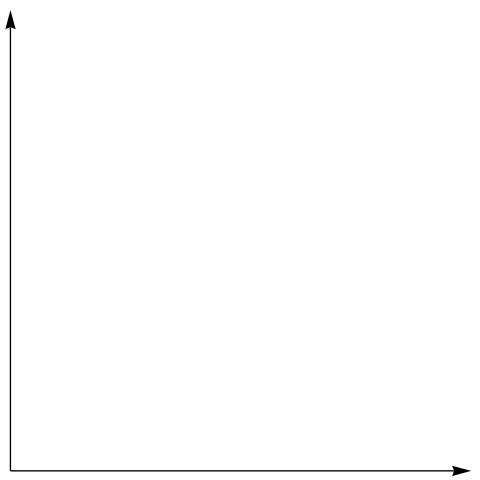
\includegraphics[width=\textwidth]{Steinitz1}
            \caption{$X$}
        \end{subfigure}
        \hfill
        \begin{subfigure}[b]{0.45\textwidth}
            \centering
            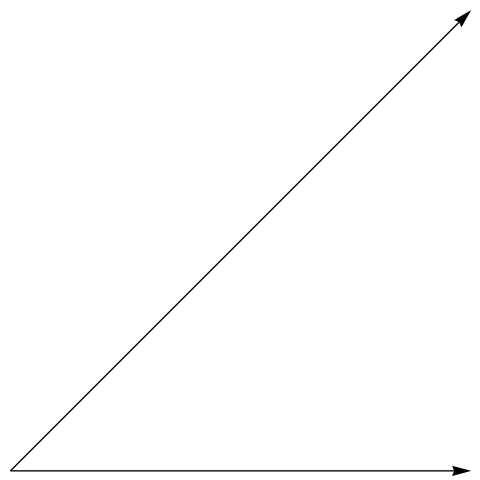
\includegraphics[width=\textwidth]{Steinitz2}
            \subcaption{$Y$}
        \end{subfigure}
        \caption{Steinitz exchange lemma says you can swap a vector in a basis so long as it preserves the span.}
        \label{fig: Steinitz Exchange Lemma}
    \end{figure}
\end{example}
Steinitz exchange lemma gives justification as to well-definededness of the notion of dimension.
\begin{definition}[Dimension]
    For finite dimensional vector space $V$,
    \textbf{dimension} of $V$, denoted as $\dim V$ is the size of any basis of $V$.
\end{definition}
\begin{exercise}
    Show that
    \begin{itemize}
        \item $\R^n$ has dimension $n$.
        \item space of polynomial of degree upto $n$ has dimension $n+1$.
        \item space of matrices $\R^{m \times n}$ has dimension $mn$.
    \end{itemize}
\end{exercise}
\begin{definition}[Row Space and Rank]
    Given $A \in \R^{m \times n}$, 
    the span of the rows of $A$ is \textbf{row space}, and
    \textbf{row rank} is defined as the dimension of the row space.
\end{definition}
\begin{exercise}
    Show that the row rank of the following matrix is 3:
    \begin{equation*}
        \begin{pmatrix}
            3 & 1 & 2 \\
            1 & 2 & 1 \\
            4 & 2 & 1 \\
            1 & 0 & -3 \\
            -2 & -3 & 0
        \end{pmatrix}
    \end{equation*}
    (Hint: EROs do not change the row space by Steinitz exchange lemma!)
\end{exercise}
\begin{exercise}
    Show that if $U \leq V$ where $V$ is finite dimensional, then
    \begin{itemize}
        \item $\dim U \leq \dim V$
        \item If $\dim U = \dim V$, then $U = V$.
    \end{itemize}
\end{exercise}
\begin{exercise}[Extension of Subspace Basis to Vector Space Basis]
    Show that if $V$ is finite dimensional and $U \leq V$, then
    any basis of $U$ can be extended to the basis of $V$.
    
    Show by an example that $U \leq V$ does not imply that basis of $V$  includes a basis of $U$.
\end{exercise}
\begin{exercise}[Dimension Formula]
    Show that $U,W \leq V$ ($V$ finite dimensional vector space), then
    $\dim \left( U+W \right) + \dim \left( U \cap W \right) = \dim U + \dim W$
\end{exercise}
\begin{example}[Dimension Formula]
    Consider $U = \spantext \left( \left\{ e_1 \right\} \right)$ and $W = \spantext \left( \left\{ e_1, e_1 + e_2 \right\} \right)$.
    Then $U + W = \R^2$, so $\dim \left( U + W \right) = 2$,
    and $U \cap V = U$, so $\dim \left( U \cap V \right) = 1$.
    This satisfies the dimension formula.
\end{example}
\begin{exercise}
    Using dimension formula or otherwise\footnote{Another way to argue is to consider the bases of the two subspaces, put them in a matrix, and note that the matrix is ``fat'', meaning it must have free variable in a matrix equation.},
    show that given $V_1, V_2 \leq V$, $\dim V_1 + \dim V_2 > \dim V$,
    $\dim \left( V_1 \cap V_2 \right) \geq 1$.
\end{exercise}
\begin{definition}[Diricet Sum]
    If $U,W \leq V$ where $V$ is finite dimensional vector space,
    and $U+W = V$, then $V$ is a \textbf{direct sum} of $U$ and $W$, and
    we write $V = U \oplus W$.
    (See Figure \ref{fig: Direct Sum})
\end{definition}
\begin{example}[Direct Sum]
    Let $V = \R^3$.
    Take $U = \spantext \left( \left\{ \left( 1, 1, 0 \right)^T \right\} \right)$,
    and $W = \spantext \left( \left\{ \left( 1, 1, 1 \right)^T, \left( 0, 1, 0 \right)^T \right\} \right)$.
    Then $V = U \oplus W$.
    \begin{figure}[h]
        \centering
        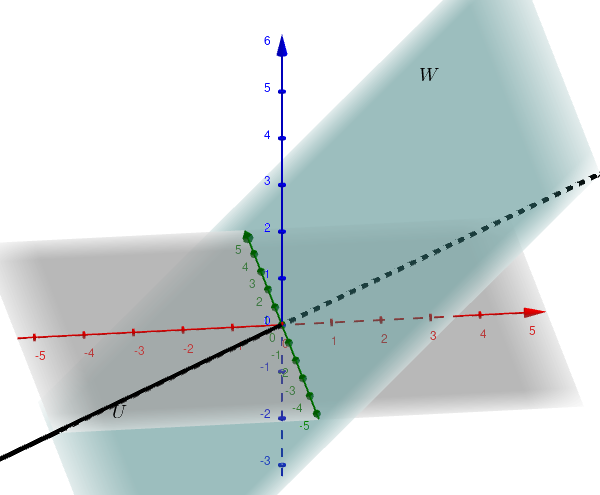
\includegraphics[scale=0.4]{DirectSum}
        \caption{$U$ and $W$ form direct sum of $V$ as the only intersection is the origin.}
        \label{fig: Direct Sum}
    \end{figure}
\end{example}
\begin{exercise}[Characterization of Direct Sum]
    Show that the following are equivalent:
    \begin{itemize}
        \item $V = U \oplus W$
        \item Every $v \in V$ has unique expression $v = u+w$ where $u \in U$ and $w \in W$.
        \item $\dim V = \dim U + \dim W$ and $V = U + W$
        \item $\dim V = \dim U + \dim W$ and $U \cap W = \left\{ 0_V \right\}$
        \item Given bases $\mathcal{B}_U$ of $U$ and $\mathcal{B}_W$ of $W$, $\mathcal{B}_U \cap \mathcal{B}_W$ is a basis of $V$.
    \end{itemize}
\end{exercise}
\begin{exercise}
    Find an example that shows $V = U \oplus W$ does not imply every basis of $V$ is a union of basis of $U$ and a basis of $W$.
\end{exercise}

\section{Linear Transformation}
Linear transformation is the reason why we define matrix multiplication in such a funky way.
\begin{definition}[Linear Transformation]
    Let $V, W$ be vector spaces over $\mathbb{F}$.
    Map $T: V \rightarrow W$ is a \textbf{linear transformation} if
    \begin{itemize}
        \item $T\left( v_1 + v_2 \right) = T\left( v_1 \right) + T\left( v_2 \right)$.
        \item $T\left( \lambda v \right) = \lambda T\left( v \right)$.
    \end{itemize}
\end{definition}
\begin{remark}
    It is as if $T$ can be replaced by a matrix\dots Hm\dots
\end{remark}
\begin{example}
    \begin{itemize}
        \item Identity map $\text{id}_V:V \rightarrow V$ defined by $\text{id}_V (v) = v$ is a linear map.
        \item Zero map $z:V \rightarrow W$ defined by $z(v) = 0$ is a linear map.
        \item Given a matrix $A \in \R^{m \times n}$, left multiplication map $L:\R^n \rightarrow \R^m$ defined by $L(v) = Av$ is a linear map.
        \item Given $V = U \oplus W$, we know we can uniquely write $v = u + w$ where $u \in U$ and $w \in W$. Projection map $P:V \rightarrow V$ defined by $P(v) = w$ is a linear map.
    \end{itemize}
\end{example}
\begin{exercise}
    Given $U, V, W$ be vector spaces, if $S:U \rightarrow V$ and $T:V \rightarrow W$ are linear,
    then $TS \coloneqq T \circ S:U \rightarrow W$ is also a linear transformation.
\end{exercise}
\begin{exercise}
    \label{ex: Linear Transform Determined By Image of Basis}
    Given $U, V$ be vector spaces, show that linear map $T:U \rightarrow V$ is uniquely defined by
    the image of $T$ for a basis of $U$, that is,
    if $\left\{ u_1, \cdots, u_m \right\}$ is a basis of $U$, 
    map is uniquely determined provided the outputs of $T\left( u_i \right)$.
\end{exercise}
\begin{remark}[Matrix Multiplication and Linear Transform]
    \label{rmk: Matrix Multiplication and Linear Transform}
    \textbf{This was a revelation for me when I learned this.}
    Consider matrix
    \begin{equation*}
        A =
        \begin{pmatrix}
            1 & 2 & 3 \\
            4 & 5 & 6 \\
            7 & 8 & 9
        \end{pmatrix}
    \end{equation*}
    Then notice that $Ae_1 = \left( 1,4,7 \right)^T$,
    $Ae_2 = \left( 2,5,8 \right)^T$,
    and $Ae_3 = \left( 3,6,9 \right)^T$.
    Note that these are columns of the matrix $A$.
    Now consider
    \begin{equation*}
        A
        \begin{pmatrix}
            1 \\ 2 \\ 3
        \end{pmatrix}
        = A \left( e_1 + 2 e_2 + 3 e_3 \right)
        =
        \begin{pmatrix}
            1 \\ 4 \\ 7
        \end{pmatrix}
        +
        2
        \begin{pmatrix}
            2 \\ 5 \\ 8
        \end{pmatrix}
        +
        3
        \begin{pmatrix}
            3 \\ 6 \\ 9
        \end{pmatrix}
    \end{equation*}
    This and Exercise \ref{ex: Linear Transform Determined By Image of Basis} suggests that
    \textbf{any linear map in a finite dimensional vector space can be written as a left matrix multiplication.}
    This is also why I stick by remark \ref{rmk: Column Vector},
    unless you know for sure that you will be working with right multiplication.
\end{remark}
\begin{example}
    To describe a counterclockwise rotation by angle $\theta$ in $\R^2$,
    note that we can map 
    $
    \begin{pmatrix}
        1 \\ 0
    \end{pmatrix}
    \mapsto
    \begin{pmatrix}
        \cos \theta \\ \sin\theta
    \end{pmatrix}
    $,
    and
    $
    \begin{pmatrix}
        0 \\ 1
    \end{pmatrix}
    \mapsto
    \begin{pmatrix}
        -\sin\theta \\ \cos\theta
    \end{pmatrix}
    $
    .
    This linear transform can be described by a left multiplication by the orthogonal matrix:
    \begin{equation*}
        Tv \coloneqq
        \underbrace{
        \begin{pmatrix}
            \cos \theta & -\sin \theta \\
            \sin \theta & \cos \theta
        \end{pmatrix}
    }_{\text{orthogonal}}
        v
    \end{equation*}
    Check again that it maps the basis $e_1, e_2$ to their respective images.
\end{example}
\begin{exercise}
    Construct a linear map in $\R^3$ that describes $\frac{2\pi}{3}$ rotation around the axis $\left( 1,1,1 \right)^T$.
\end{exercise}
\begin{remark}
    While it is helpful to get intuition in terms of canonical basis,
    left multiplication by matrix describes linear transformation in any given basis in their ``coordinates''.
    See Example \ref{eg: Change of Basis}.
\end{remark}
\subsection{Rank and Nullity}
\begin{definition}[Kernel and Image]
    Given $V, W$ to be vector spaces and $T:V \rightarrow W$ is linear,
    \textbf{kernel} (null space) of $T$ is
    \begin{equation*}
        \ker T \coloneqq \left\{ v \in V \middle| T(v) = 0_W \right\}
    \end{equation*}
    and \textbf{image} of $T$ is
    \begin{equation*}
        \im T \coloneqq \left\{ T(v) \middle| v \in V \right\}
    \end{equation*}
\end{definition}
\begin{remark}
    Kernel is the set of vectors that map to zero.
    Image is the set of vectors that end up being mapped to from $V$.
\end{remark}
\begin{exercise}
    For $V, W$ vector spaces and $T:V \rightarrow W$ linear,
    $T$ is injective if and only if $\ker T = \left\{ 0_V \right\}$.
\end{exercise}
\begin{exercise}[Kernel and Image are Subspaces]
    For $V, W$ vector spaces and $T:V \rightarrow W$ linear, show
    \begin{itemize}
        \item $\ker T \leq V$ and $\im T \leq W$
        \item if $\left\{ v_1, \cdots, v_m \right\}$ spans $V$, then $T(\left\{ v_1, \cdots, v_m \right\})$ spans $\im T$
    \end{itemize}
\end{exercise}
Since the kernel and image are subspaces, we are interested in their dimensions.
\begin{definition}[Rank and Nullity]
    $V, W$ being vector spaces with $V$ finite dimensional.
    $T: V \rightarrow W$ linear.
    \begin{itemize}
        \item \textbf{Nullity} of $T$ is $\Null T \coloneqq \dim \left( \ker T \right)$
        \item \textbf{Rank} of $T$ is $\Rank T \coloneqq \dim \left( \im T \right)$
    \end{itemize}
\end{definition}
\begin{exercise}[Rank-Nullity Theorem]
    Given $V, W$ being vector spaces with $V$ finite dimensional, and
    $T: V \rightarrow W$ linear,
    show that $\dim V = \Rank T + \Null T$
\end{exercise}

\section{Change of Basis}
It was already mentioned at remark \ref{rmk: Matrix Multiplication and Linear Transform} that
matrix can be used to describe a linear map 
\textbf{Note that in the discussion we were implicitly assuming that we were using canonical basis}\footnote{
    The use of canonical basis seems like a natural choice, but from the POV of mathematics,
    it is an arbitrary choice\dots, like we use canonical basis only because they are easy to compute,
    most of the times.
}.
Now we want to see the relationship between two matrices describing the same linear tranform,
but in different basis.
\begin{example}
    \label{eg: Change of Basis}
    Consider linear map $T:\R^2 \rightarrow \R^2$ defined as $T(x,y) = 
    \begin{pmatrix}
        2x + y\\
        3x - 2y
    \end{pmatrix}
    $.
    Note that
    \begin{align*}
        T\left( 1,0 \right) = 
        \begin{pmatrix}
            2 \\ 3
        \end{pmatrix}
        &&
        T\left( 0,1 \right) = 
        \begin{pmatrix}
            1 \\ -2
        \end{pmatrix}
    \end{align*}
    So with respect to basis $e_1, e_2$, the matrix describing this transformation is
    \begin{equation*}
        A =
        \begin{pmatrix}
            2 & 1\\ 3 & -2
        \end{pmatrix}
    \end{equation*}
    On the other hand, consider another basis $f_1 = \left( 1, -2 \right)^T, f_2 = \left( -2, 5 \right)^T$ of $\R^2$.
    Then
    \begin{align*}
        T\left( f_1 \right) = 
        \begin{pmatrix}
            0 \\ 7
        \end{pmatrix}
        =
        14 f_1 + 7 f_2
        &&
        T\left( f_2 \right) = 
        \begin{pmatrix}
            1 \\ -16
        \end{pmatrix}
        = -27f_1 - 14f_2
    \end{align*}
    So with respect to basis $f_1, f_2$, the matrix describing this transformation is
    \begin{equation*}
        B =
        \begin{pmatrix}
            14 & -27 \\
            7 & -14
        \end{pmatrix}
    \end{equation*}

    These two matrices describe the \textit{same} linear transform, just in different basis.
    We can actually explicitly construct how they are related.

    \textbf{Idea}: Change basis from one to the other, perform the transform in the new basis, and turn it back to the original basis.
    Because of the relation of the two bases:
    \begin{align*}
        f_1 &= e_1 - 2e_2 \\
        f_2 &= -2e_1 + 5e_2
    \end{align*}
    Construct the change of basis matrix $P$, ``used for mapping from $f_i$ coordinates to $e_i$ coordinates:
    \begin{equation*}
        P =
        \begin{pmatrix}
            1 & -2 \\ -2 & 5
        \end{pmatrix}
    \end{equation*}
    The inverse matrix describes the mapping from $e_i$ coordinates to $f_i$ coordinates.
    \begin{equation*}
        P^{-1} =
        \begin{pmatrix}
            5 & 2 \\ 2 & 1
        \end{pmatrix}
    \end{equation*}
    Then it must be that $P^{-1}AP$ describes the linear transformation in $f_i$ coordinates\footnote{
        In more detail, $P$ first maps from $f_i$ coordinates to $e_i$ coordinates.
        Then $A$ does the actual linear map in $e_i$ coordinates.
        Finally $P^{-1}$ maps the coordinates in $e_i$ to ones in $f_i$.
    },
    hence $P^{-1}AP = B$.
    (Indeed you can verify this.)
\end{example}
\begin{remark}
    Explicit construction of $A = P^{-1}BP$ is not really the highlight of the course,
    but it is worth understanding the process.
\end{remark}
\begin{definition}[Similarity]
    If there exists invertible $P\in\R^{n \times n}$ such that $A,B \in \R^{n \times n}$,
    then we say $A$ and $B$ are \textbf{similar}.
\end{definition}
\begin{exercise}[Similarity is an Equivalence Relation]
    Verify that similarity is an equivalence relation by checking the three conditions of equivalence relation.
\end{exercise}

\section{Matrix and Rank}
We've seen that matrix and linear transforms are very much related.
In fact, we might as well start abusing the notion of ``rank'' of a matrix!
We do need to check if the definition of rank for a matrix is well-defineded and natural\footnote{
    Intuition may say well-defined, since change of basis does not change the actual span of them\dots
}

To do so, it helps to show one result:
\begin{exercise}
    For $A \in \R^{m \times n}$, there exists invertible $P \in \R^{n \times n}$ and $Q \in \R^{m \times m}$ 
    such that $Q^{-1}AP$ can be written as:
    \begin{equation}
        Q^{-1}AP =
        \begin{pmatrix}
            I_{r} & 0_{r \times s} \\ 0_{t \times r} & 0_{t \times s}
        \end{pmatrix}
        \label{equ: RRE/RCE}
    \end{equation}
    (Hint: The simplest argument is to note that elementary row operations are simply left multiplication by invertible matrices.
    Similarly one could consider elementary column operations, which must be right multiplication by invertible matrices.
    Then we consider the RRE/RCE\footnote{Reduce column echelon} form.
)
\end{exercise}
Using this, one could argue now the following result:
\begin{exercise}[Column Rank is Equal to Row Rank]
    Deduce from (\ref{equ: RRE/RCE}) that the column rank and the row rank of $A \times \R^{m \times n}$ are the same.
    (Hint: You can read off $r$ to be both the column rank and the row rank.)
\end{exercise}
So finally we have rank of a matrix.
\begin{definition}[Rank of a Matrix]
    \textbf{Rank of matrix} $A \in \R^{m \times n}$, denoted by $\Rank (A)$,
    is the column rank (or row rank) of $A$.
\end{definition}
\begin{remark}
    Thinking of rank of a matrix as its column rank should reminisce you of the fact that
    matrices describe linear maps. 
    (Since the image of the map by left multiplication by the matrix is the column space.)
\end{remark}

\section{Bilinear Forms and Inner Product Space}
\begin{definition}[Bilinear Form]
    Given a vector space $V$ over $\mathbb{F}$,
    a \textbf{bilinear form} on $V$ is a function $\inner{\cdot, \cdot} : V \times V \rightarrow \mathbb{F}$
    such that
    \begin{itemize}
        \item $\inner{\alpha_1 v_1 + \alpha_2 v_2, v_3} = \alpha_1 \inner{v_1, v_3} + \alpha_2 \inner{v_2, v_3}$
        \item $\inner{v_1, \alpha_2 v_2 + \alpha_3 v_3} = \alpha_2 \inner{v_1, v_2} + \alpha_3 \inner{v_1, v_3}$
    \end{itemize}
    for all $v_1, v_2, v_3 \in V$ and $\alpha_1, \alpha_2, \alpha_3 \in \mathbb{F}$
\end{definition}
\begin{remark}
    Bilinear form is a generalization of dot product in a way.
    In fact, $\inner{x, y} = x^T y$ (usual dot product) for $x, y \in \R^n$ over $\R$ is indeed a bilinear form.
\end{remark}
\begin{example}
    Given $A \in \mathbb{F}^{n \times n}$, $\inner{x, y} \coloneqq x^T A y$ is a bilinear form over $\mathbb{F}$.
\end{example}
\begin{definition}[Inner Product Space]
    Bilinear form $\inner{\cdot, \cdot} : V \times V \rightarrow \mathbb{R}$ is
    \begin{itemize}
        \item \textbf{symmetric} if
            $\inner{v_1, v_2} = \inner{v_2, v_1}$ for all $v_1, v_2 \in V$.
        \item 
            \textbf{positive definite} if
            $\inner{v, v} \geq 0$ for all $v \in V$ where equality if and only if $v = 0$.
    \end{itemize}
    \textbf{Inner product space} is a positive definite symmetric bilinear form on $V$.
\end{definition}
\begin{remark}
    Dot product is still an inner product over $\mathbb{R}^n$.
\end{remark}
\begin{definition}
    For real inner product space $V$, define \textbf{norm} of $v \in V$ is
    \begin{equation*}
        \norm{v} \coloneqq \sqrt{\inner{v,v}}
    \end{equation*}
\end{definition}
\begin{exercise}
    \label{ex: Polynomial Inner Product}
    Consider $V = \R_n \left[ x \right]$, a space of polynomials of degree $n$ with real coefficients.
    Show that $\inner{f, g} \coloneqq \int_{-1}^1 f(x) g(x) \intd x$ is an inner product over $V$.
\end{exercise}
Often we are interested in orthonormal set, as it makes the computation much easier.
\begin{definition}[Orthonormal Set]
    Given $V$ an inner product space, $\left\{ v_1, \cdots, v_n \right\} \subset V$ is an \textbf{orthonormal set}
    if for all $i,j$,
    \begin{equation*}
        \inner{v_i, v_j} = \delta_{i,j}
    \end{equation*}
\end{definition}
\begin{exercise}
    $\left\{ v_1, \cdots, v_n \right\}$ be an orthonormal set in an inner product space $V$.
    Then show that $v_1, \cdots, v_n$ are linear independent.
\end{exercise}
\begin{exercise}
    Show that canonical basis of $\R^n$ is an orthonormal set.
\end{exercise}
\begin{exercise}[Legendre Polynomials]
    Construct an orthonormal set of basis for the inner product space for $\mathbb{R}_2 \left[ x \right]$.
\end{exercise}
\begin{exercise}[Orthogonality in Fourier Series]
    For what $k>0$ is the set $\left\{ \cos{(nx)} \middle| n = 1, 2, \cdots \right\}$ an orthonormal set
    under inner product $\inner{f,g} \coloneqq \int_{-\pi}^\pi f(x) g(x) \intd x$?
\end{exercise}

\subsection{Orthogonal Matrices}
\begin{definition}[Orthogonal Matrix]
    $Q \in \R^{n \times n}$ is an \textbf{orthogonal matrix} if $Q^T Q = Q Q^T = I$.
    In other words, $Q^T = Q^{-1}$.
\end{definition}
\begin{exercise}[Characterization of Orthogonal Matrices]
    Show that orthogonal matrices can be characterized in any of the following ways:
    \begin{itemize}
        \item $Q Q^T = I$
        \item $Q^T Q = I$
        \item Rows of $Q$ form an orthonormal basis of $\R^n$.
        \item Columns of $Q$ form an orthonormal basis of $\R^n$.
        \item $\left( Q x \right)^T \left( Q y \right) = x^T y$ for all $x, y \in \R^n$
    \end{itemize}
\end{exercise}
\begin{exercise}
    Deduce that the Euclidean norms of each row and column are 1.
\end{exercise}
\begin{exercise}
    If $U,V \in \R^{n \times n}$ are both orthogonal matrices, show that $UV$ is also an orthogonal matrix.
\end{exercise}

\section{Cauchy Schwarz Inequality}
Here is a theorem that is actually used a lot, like for constructing an upper bound.
\begin{exercise}[Cauchy Schwarz Inequality]
    Show the following:
    For $V$ real inner product space, $|\inner{v_1, v_2}| \leq \norm{v_1} \norm{v_2}$
    with equality if and only if $v_1, and v_2$ are linearly dependent.
    
    (Hint: Consider $\inner{tv_1 + v_2, tv_1 + v_2}$, and note that it is nonnegative for all $t \in \R$.)
\end{exercise}
\begin{exercise}
    Show using Cauchy Schwarz inequality that,
    given $U \leq \R^n$,
    the minimization problem ($a \in U$ is given):
    \begin{equation*}
        \min_{x \in \R^n} \norm{x - a}
    \end{equation*}
    is solved by taking $x$ such that $\inner{x - a, r} = 0$ for all $r \in U$.
    (Hint: Consider $\norm{x-a}^2 = \inner{x - a, x-r} + \inner{x-a, r-p}$ for any $r \in U$)
    What does this mean geometrically?\footnote{Something about projection onto $U$?}
\end{exercise}
\section{Complex Inner Product Space}
One can generalize the real inner product space to complex inner product by considering
sesquilinear form.
\begin{definition}[Sesquilinear Form]
    Given a vector space $V$ over $\mathbb{C}$,
    a \textbf{sesquilinear form} on $V$ is a function $\inner{\cdot, \cdot} : V \times V \rightarrow \mathbb{C}$
    such that
    \begin{itemize}
        \item $\inner{\alpha_1 v_1 + \alpha_2 v_2, v_3} = \alpha_1 \inner{v_1, v_3} + \alpha_2 \inner{v_2, v_3}$
        \item $\inner{v_1, v_2} = \overline{\inner{v_2, v_1}}$.
    \end{itemize}
    for all $v_1, v_2, v_3 \in V$ and $\alpha_1, \alpha_2, \alpha_3 \in \mathbb{C}$
\end{definition}

\part{Linear Algebra II}
\section{Determinants}
Determinant characterizes the overall ``scalar stretch'' by a square matrix.
(Consider the eigenvalues, which will be covered in the later section.)
\begin{definition}[Determinant]
    Given $A = 
    \begin{pmatrix}
        a_1 & \cdots & a_n
    \end{pmatrix}
    \in \R^{n \times n}$
    where $a_i$ are the columns,
    define the \textbf{determinantal map} $D : \R^{n \times n} \rightarrow \R$ as:
    \begin{itemize}
        \item Multilinear in columns:
            \begin{itemize}
                \item $D \left[ \cdots, b_i + c_i, \cdots \right] = D \left[ \cdots, b_i, \cdots \right] + D \left[ \cdots, c_i, \cdots \right]$
                \item $D \left[ \cdots, \lambda a_i, \cdots \right] = \lambda D \left[ \cdots, a_i, \cdots \right]$
            \end{itemize}
        \item Alternating: $D[\cdots, a_i, a_{i+1}, \cdots] = 0$ if $a_i = a_{i+1}$
        \item $D\left( I \right) = 0$
    \end{itemize}
    \textbf{Determinant} of matrix $A$ is then $D(A)$.
\end{definition}
\begin{exercise}
    Show that the determinant of $
    \begin{pmatrix}
        a & b \\ c & d
    \end{pmatrix} = ad-bc
    $
    only using the definition of a determinantal map.
\end{exercise}
\begin{exercise}
    A more useful way to compute the determinant is to use the Laplace expansion:
    \begin{equation*}
        \det (A) = \sum_{\sigma \in S_n} \sgn \left( \sigma \right) a_{\sigma(1), 1} \cdots a_{\sigma(n),n}
    \end{equation*}
    Use this expansion formula to compute the determinant of $
    \begin{pmatrix}
        a & b & c \\
        d & e & f \\
        g & h & i
    \end{pmatrix}
    $
    (Note that you will be summing over 6 terms in total, since $|S_3| = 6$)
\end{exercise}
\begin{exercise}
    Show that $\det (A) = \det \left( A^T \right)$.
    (Hint: $\sgn{\sigma} = \sgn{\left( \sigma^{-1} \right)}$.)
\end{exercise}
It turns out that determinant is multiplicative, as in:
\begin{equation*}
    \det \left( AB \right) = \det \left( A \right) \det \left( B \right)
\end{equation*}
One way to prove this is to use the fact that we basically know
how the determinant changes through EROs/ECOs.
\begin{exercise}
    Deduce that noninvertible matrix has zero determinant.
\end{exercise}
\begin{exercise}
    Deduce that if $A$ is invertible, then $\det \left( A^{-1} \right) = \frac{1}{\det \left( A \right)}$
\end{exercise}
\begin{exercise}
    Consider linear map $T$. Show that in two bases $\mathcal{B}_1$ and $\mathcal{B}_2$,
    the matrices describing $T$ have the same determinants.
\end{exercise}
\section{Eigenvectors and Eigenvalues}
Eigenvalues (and other eigenstuff) are very important property of linear maps and matrices.
\begin{definition}[Eigenvalue and Eigenvectors]
    Consider linear map $T : V \rightarrow V$.
    $v \in V$ is an \textbf{eigenvector} of $T$ if $v \neq 0$ and $Tv = \lambda v$ for some $\lambda \in \mathbb{C}$.
    $\lambda$ is the corresponding \textbf{eigenvalue} to the eigenvector.
\end{definition}
\begin{figure}[h]
    \centering
    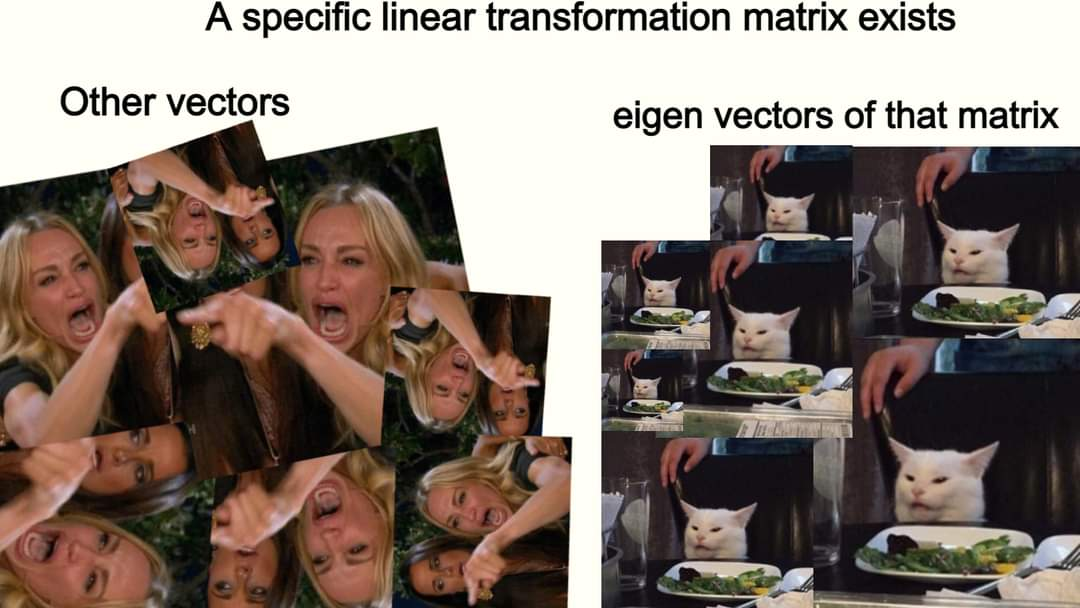
\includegraphics[width=0.7\textwidth]{EigenvectorMeme}
    \caption{A meme about eigenvectors.}
    \label{fig: Eigenvector Meme}
\end{figure}
\begin{remark}
Eigenvectors are the vectors experiencing only ``stretching'', not rotation or otherwise.
(See Figure \ref{fig: Eigenvector Meme})
Note that \textbf{eigenvectors cannot be zero vectors} even though $\lambda$ could be zero.
\end{remark}
\begin{example}
    Identity matrix $I \in \R^{n \times n}$ satisfies:
    \begin{align*}
        Iv = 1v
    \end{align*}
    for all $v \in \R^n$, so any nonzero vector $v \in \R^n$ is an eigenvector of $I$,
    with corresponding eigenvalue 1.
\end{example}
\begin{exercise}
    Find eigenvectors corresponding to $\pm i$ for
    \begin{equation*}
        \begin{pmatrix}
            0 & -1 \\ 1 & 0
        \end{pmatrix}
    \end{equation*}
    (Note that there are infinite eigenvectors since if $v$ is an eigenvector, $kv$ is also an eigenvector of the same eigenvalue for any $k \in \R \setminus \left\{ 0 \right\}$)
\end{exercise}
\begin{exercise}[Eigenvalue of Inverse Matrix]
    Given an invertible matrix $A \in \R^{n \times n}$ and writing the spectrum\footnote{Multiset of eigenvalues} of it as $\lambda_1, \cdots, \lambda_n$,
    what is the spectrum of $A^{-1}$? What are the corresponding eigenvectors?
\end{exercise}
\begin{exercise}[Eigenvalues Shifted]
    Suppose $A \R^{n \times n}$ has spectrum $\lambda_1, \cdots, \lambda_n$.
    Show that the spectrum of $A - \mu I$ is $\lambda_1 -\mu, \cdots, \lambda_n - \mu$, where $\mu$ is a constant.
\end{exercise}
\begin{exercise}[Modulus of Eigenvalues of Orthogonal Matrices is 1]
    Suppose $A \in \R^{n \times n}$ is an orthogonal matrix and $\lambda$ is an eigenvalue of $A$.
    Show that $|\lambda|=1$
    (Hint: Consider $\left( Av \right)^{*} \left( Av \right)$ where $*$ represents conjugate transpose. Note that while $A$ is a real matrix, $v$ can be complex. You might also find the property $u^* u = \norm{u}^2$ for any $u \in \R^n$ useful.)
\end{exercise}
\begin{exercise}
    Show that $\lambda$ is an eigenvalue of linear map $T$, if and only if $\ker {\left( T - \lambda I \right)} \neq \left\{ 0 \right\}$.
    (Hint: This characterization basically says $\left( T - \lambda I \right)v = 0$ must have nontrivial solution $v$.)
\end{exercise}
\begin{exercise}[Further Characterizations of Eigenvalue]
    Show that $\lambda$ being an eigenvalue of $T$ is also equivalent to any of the following:
    \begin{itemize}
        \item $T - \lambda I$ is not invertible.
        \item $\det \left( T - \lambda I \right) = 0$
    \end{itemize}
\end{exercise}

To find eigenvalue, one could turn it into a root finding problem:
\begin{definition}[Characteristic Polynomial]
    For $A \in \R^{n \times n}$, \textbf{characteristic polynomial} is defined as $\chi ( \lambda ) = \det \left( A - \lambda I \right)$
    For a linear map $T$, it is defined as $\det \left( A - \lambda I \right)$ where $A$ is matrix describing the linear map in any basis. (This is well-defined since $\det \left( P^{-1} A P \right) = \det \left( A \right)$)
\end{definition}
\begin{exercise}[Roots of Characteristic Polynomials are Eigenvalues]
    Show that $\lambda$ is an eigenvalue of linear map $T$ if and only if it is the root of its characteristic polynomial.
\end{exercise}
\begin{exercise}[Companion Matrix]
    Consider the polynomial $p(x) = c_0 + c_1 x + \cdots + c_{n-1} x^{n-1} + x^n$ and the
    following matrix (called the companion matrix):
    \begin{equation*}
        C =
        \begin{pmatrix}
            0 & 1 & 0 & \cdots & 0 \\
            0 & 0 & 1 & \cdots & 0 \\
            \vdots & \vdots & \vdots & \ddots & \vdots \\
            0 & 0 & 0 & \cdots & 1 \\
            -c_0 & -c_1 & -c_2 & \cdots & -c_{n-1}
        \end{pmatrix}
    \end{equation*}
    Show that the characteristic polynomial of $C$ is $p(x)$, and hence show that there is no way to express exactly the eigenvalues of general $n \times n$ matrices ($n \geq 5$).
\end{exercise}
\begin{exercise}[Characteristic Polynomial Evaluation]
    (Maybe not terribly important, but) show that for linear map $T$ and its characteristic polynomial $\chi (\lambda)$,
    \begin{equation*}
        \chi (T) = 0
    \end{equation*},
    that is $\chi (T)$ is a zero map.
\end{exercise}
\begin{exercise}
    Show that if $\lambda$ is a nonreal, complex eigenvalue of linear map $T:\R^n \rightarrow \R^n$, then $\bar{\lambda}$ must also be an eigenvalue.
\end{exercise}
\begin{exercise}
    Show that for $A \in \R^{n \times n}$,
    \begin{equation*}
        \chi (\lambda) = \left( -1 \right)^n \lambda^n + \left( -1 \right)^{n-1} \tr \left( A \right) \lambda^{n-1} + \cdots + \det \left( T \right)
    \end{equation*}
\end{exercise}
\begin{remark}
    This shows that for $A \in \R^{n \times n}$
    \begin{equation*}
        | \det {T} | = \left| \prod_{i=1}^n \lambda_i \right|
    \end{equation*}
    where $\lambda_i$ are eigenvalues of $A$ (with multiplicity).
    This suggests that determinant is the overall stretch,
    and eigenvalues are stretches that make up the overall stretch.
    \begin{figure}[tbp]
        \centering
        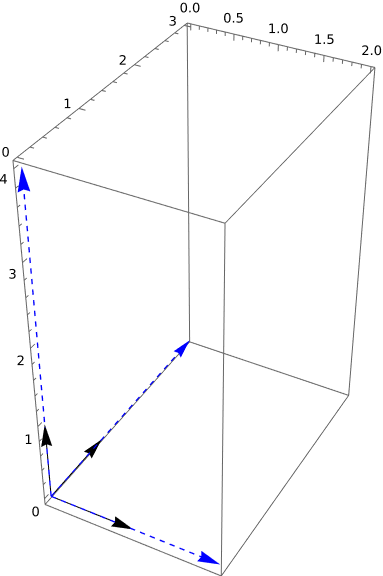
\includegraphics{EigenvalueDeterminant}
        \caption{Map of $e_1, e_2, e_3$ (black) under left-multiplication by $\diag \left( 2, 3, 4 \right)$, which has eigenvalues 2, 3, and 4, and the corresponding eigenvectors are $e_1, e_2, e_3$ respectively. Resulting vectors are drawn in blue.}
        \label{fig: EigenvalueDeterminant}
    \end{figure}
    See Figure \ref{fig: EigenvalueDeterminant} for a small demonstration of this.
\end{remark}
\begin{exercise}
    Show that if $\lambda_1, \cdots, \lambda_m$ ($m \neq n$) are distinct eigenvalues of $T$ with
    corresponding eigenvectors being $v_1, \cdots, v_m$, then
    $v_1, \cdots, v_m$ is linearly independent.
\end{exercise}

\section{Diagonalization}
Note that eigenvectors look like something we could use as a basis.
In fact, using eigenvectors as basis has the benefit of simplfying the computation much easier.
However we need to worry if we can even have eigenvectors as basis in the first place.
This is where the idea of diagonalizability comes in.

\begin{definition}[Diagonalizability]
    Linear map $T :V \rightarrow V$ is \textbf{diagonalizable} if $V$ has a basis consisting of eigenvectors for $T$.
\end{definition}
\begin{remark}
    While the original definition of diagonalizability may not make sense as to why it is called diagonalizability,
    it is because if you were to write $T$ as a matrix in the eigenvector basis, you would end up with a diagonal matrix.
\end{remark}
\begin{exercise}
    Matrix $A \in \R^{n \times n}$ is diagonalizable if and only if there exists invertible $P$ such that $B \coloneqq P^{-1} A P$ is a diagonal matrix (with columns of $P$ being the eigenvectors)
    (Hint: Submatrix multiplication might be useful?)
\end{exercise}
\begin{exercise}
    Deduce that if linear map $T:V \rightarrow V$ had $n$ distinct eigenvalues, it is diagonalizable.
    Is the converse true?
\end{exercise}
\begin{exercise}
    Given a diagonalizable matrix
    \begin{equation*}
        A =
        \begin{pmatrix}
            0 & -2 \\ 1 & 3
        \end{pmatrix}
    \end{equation*}
    find $P,\Lambda \in \R^{2 \times 2}$ such that $A = P^{-1} D P$,
    where $D$ is a diagonal matrix.
    Is this decomposition unique?
\end{exercise}

\subsection{Geometric and Algebraic Multiplicity}
\begin{definition}[Eigenspace]
    Let $\lambda$ be an eigenvalue of $T$.
    \textbf{Eigenspace} for $\lambda$ is
    \begin{equation*}
        E_{\lambda} = \left\{ v \in V : Tv = \lambda v \right\}
    \end{equation*}
\end{definition}
\begin{remark}
    Eigenspace for $\lambda$ is the span of all eigenvectors with eigenvalue $\lambda$.
\end{remark}
\begin{definition}[Multiplicity]
    Let $\lambda$ be eigenvalue of $T$.
    Then \textbf{geometric multiplicity} of $\lambda$ is $\dim E_{\lambda}$,
    and \textbf{algebraic multiplicity} of $\lambda$ is the multiplicity of $\lambda$ as a root of characteristic polynomial $\chi \left( \lambda \right)$.
\end{definition}
\begin{exercise}
    Show that geometric multiplicity of $\lambda$ is less than or equal to its algebraic multiplicity.
\end{exercise}
\begin{exercise}
    Show that given $\lambda_1, \cdots, \lambda_r$ ($r \neq n$) which are distinct eigenvalues of $T$,
    $E_{\lambda_1}, \cdots, E_{\lambda_r}$ form direct sum.
\end{exercise}

\section{Spectral Theorem}
Given basis $v_1, \cdots, v_n$ (not necessarily orthogonal) in a real inner product space $V$,
one can construct orthogonal basis $u_1, \cdots, u_n$ through Gram-Schmidt procedure.
\begin{align*}
    u_k = \frac{v_k - \sum_{i=1}^{k-1} \inner{v_k, u_i}u_i}{\norm{v_k - \sum_{i=1}^{k-1} \inner{v_k, u_i}u_i}}
\end{align*}
To understand this, note that $\inner{v_k, u_i}$ picks out the ``component'' of $v_k$ in the $u_i$ direction.
One could subtract off all these vectors out to get a vector that is orthogonal to all the previous ones.
\begin{example}
    Given the basis of $\R^3$
    \begin{equation*}
        \begin{pmatrix}
            1 \\ 0 \\ 0
        \end{pmatrix},
        \begin{pmatrix}
            1 \\ 1 \\ 1
        \end{pmatrix},
        \begin{pmatrix}
            3 \\ 2 \\ 1
        \end{pmatrix}
    \end{equation*}
    construct an orthogonal set of basis using Gram-Schmidt. (In the usual dot product)
\end{example}
\begin{example}
    Use Gram-Schmidt to construct orthogonal basis from:
    \begin{equation*}
        \begin{pmatrix}
            1 \\ 1 \\ 1
        \end{pmatrix},
        \begin{pmatrix}
            3 \\ 2 \\ 1
        \end{pmatrix},
        \begin{pmatrix}
            4 \\ 1 \\ 2
        \end{pmatrix}
    \end{equation*}
    with inner product defined as:
    \begin{equation*}
        \inner{
            \begin{pmatrix}
                x_1 \\ x_2 \\ x_3
            \end{pmatrix},
            \begin{pmatrix}
                y_1 \\ y_2 \\ y_3
            \end{pmatrix}
        }
        \coloneqq
        x_1 y_1 + 2 x_2 y_2 + x_3 y_3
    \end{equation*}
    (This question was asked on Stack Overflow, which I've provided the solution to with Python:
    \url{https://stackoverflow.com/questions/76381803/gram-schmidt-algorithm-using-nympy-sympy-for-a-custom-inner-product-space/76385749#76385749}.)
\end{example}

\subsection{Spectral Theorem for Symmetric Matrix}
We restrict our attention to symmetric matrices of the form $A^T = A \in \R^{n \times n}$.
\begin{exercise}
    Show that all eigenvalues of symmetric matrix $A$ are real.
\end{exercise}
Finally we state the spectral theorem for symmetric matrix in the most concise way possible.
\begin{exercise}[Spectral Theorem for Symmetric Matrix]
    Prove the following statement.
    Symmetric matrix $A$ is diagonalizable over $\R^n$, and the eigenvectors form an orthogonal basis (in terms of regular dot product), in fact!
\end{exercise}
\begin{remark}
    From now on, whenever you see symmetric matrix $A$, you should immediately try writing it as the eigendecomposition $A = V \Lambda V^T$.
\end{remark}
\begin{exercise}
    Given orthogonal matrix:
    \begin{equation*}
        A =
        \begin{pmatrix}
            1 & \mu \\ \mu & 1
        \end{pmatrix}
    \end{equation*}
    where $\mu \in \R \setminus \left\{ 0 \right\}$,
    express it as $V \Lambda V^T$ where $V$ is orthogonal and $\Lambda$ is diagonal.
\end{exercise}
\begin{exercise}[SVD for Symmetric Matrix]
    For symmetric $A \in \R^{n \times n}$,
    by using the fact that there is eigendecomposition $A = P \Lambda P^T$,
    or otherwise,
    prove that there exists singular value decomposition: $A = U \Sigma V^T$,
    where $U, V$ are orthogonal matrices and $\Sigma$ is a diagonal matrix of
    \underline{nonnegative} entries.
    (Hint: This is actually really easy! Can you decompose $\Lambda$ to
    $Q \Sigma$ where $Q$ is orthogonal?)
\end{exercise}
\begin{exercise}[$A$-inner Product]
    Consider the bilinear form $\inner{\cdot, \cdot}: \R^n \rightarrow \R$ defined as
    \begin{equation*}
        \inner{x, y} \coloneqq x^T A y
    \end{equation*}
    where $A$ is a symmetric matrix.
    Show that this bilinear form is inner product if and only if $A$ only has positive eigenvalues.
\end{exercise}
\begin{exercise}[Courant-Fischer for Largest Eigenvalue]
    Given $A$ is symmetric,
    show the following:
    \begin{equation*}
        \lambda_{1} = \max_{\norm{x} = 1} x^T A x
    \end{equation*}
    where $\norm{\cdot}$ is the Euclidean norm and $\lambda_{1}$ is the largest eigenvalue of $A$.
\end{exercise}
\begin{exercise}[Gram Matrix is Positive Semidefinite]
    Given $A \in \R^n$ (not necessarily symmetric),
    show that $A^T A$ is a symmetric positive-semidefinite\footnote{eigenvalues are nonnegative} matrix.
\end{exercise}
\begin{exercise}[Courant-Fischer for Eigenvalue]
    A more general (and slightly tricky) statement to the previous exercise.
    Show the following:
    If $A$ is a symmetric matrix,
    \begin{equation*}
        \lambda_i = \max_{\substack{U \leq \R^n \\ \dim U = i}} \min_{\substack{\norm{x} = 1 \\ x \in U}} x^T A x
    \end{equation*}
    where $\lambda_i$ is the $i$\textsuperscript{th} largest eigenvalue.
\end{exercise}
\begin{exercise}
    Compute
    \begin{equation*}
        \begin{pmatrix}
            1 & 2 \\ 2 & 1
        \end{pmatrix}
        ^{100}
    \end{equation*}
\end{exercise}
\begin{exercise}[Householder Reflector]
    Take $\norm{\cdot}$ to be the Euclidean norm.
    Given $v \in \R^n$ such that $\norm{v} = 1$,
    define Householder reflector matrix as
    \begin{equation*}
        H_v \coloneqq I - 2vv^T
    \end{equation*}
    Show that
    \begin{itemize}
        \item $H_v$ is symmetric.
        \item $H_v$ is orthogonal matrix.
        \item if $v = \frac{u - w}{\norm{u - w}}$ for some $u, v \in \R^n$, then $H_{v} u = w$.
        \item eigenvalues of $H_v$ is $\left\{ \underbrace{+1, +1, \cdots, +1}_{n-1}, -1 \right\}$
    \end{itemize}
    Also any geometric intuition behind this? (It is called \underline{reflector} for a reason!)
\end{exercise}
\begin{exercise}
    For $A$ symmetric,
    express $\tr{(A^T A)}$ in terms of its eigenvalues.
\end{exercise}
\subsection{Quadrics}
This is simply the idea of getting a quadratic expressions into matrix form,
and defining new variables to analyze them easier.
\begin{example}
    Describe the shape of $x^2 + xy + y^2 = 1$.

    One could rewrite the relation as
    \begin{align*}
        1 &= 
        \begin{pmatrix}
            x & y
        \end{pmatrix}
        \underbrace{
        \begin{pmatrix}
            1 & \frac{1}{2} \\ \frac{1}{2} & 1
    \end{pmatrix}}_{\text{Symmetric}}
        \begin{pmatrix}
            x \\ y
        \end{pmatrix} \\
        &= u^T
        \begin{pmatrix}
            \frac{3}{2} & 0 \\ 0 & \frac{1}{2}
        \end{pmatrix}
        u
    \end{align*}
    where
        $u = P
        \begin{pmatrix}
            x \\ y
        \end{pmatrix}
        \in \R^{2 \times 1}$
        (Note that this is an orthogonal change of variables, so does not stretch the shape in any direction. Only rotates, reflects, etc.)
        In terms of $u$, we can read off that this is an equation of an ellipse.
\end{example}
\end{document}


